\documentclass[a4paper]{article}
\title{Assignment 2}
\author{Student: NAME SURNAME; Student's email: EMAIL@usi.ch}

%%%%%%%%%%%%%%%%%%%
% Packages
%%%%%%%%%%%%%%%%%%
\usepackage{palatino}
\usepackage{amsmath}
\usepackage{bm}
\usepackage{hyperref}
\usepackage{xcolor}
\usepackage{verbatim}
\usepackage{enumerate}
\usepackage{graphicx}
\usepackage[T1]{fontenc}
\usepackage{listings}


%%%%%%%%%%%%%%%%%%%
% Commands
%%%%%%%%%%%%%%%%%%
\newcommand{\erre}{\mathbf{R}}
\newcommand{\todo}[1]{\textcolor{red}{TODO: #1}}
\newcommand{\link}[2]{\href{#1}{\textcolor{blue}{#2}}}
\definecolor{code}{HTML}{00A99D}
\newcommand{\codeword}[1]{\texttt{\textcolor{code}{#1}}}

\begin{document}
	\maketitle
\section*{The Problem}
The CIFAR-10 dataset is a widely used collection of images in the field of com- puter vision. It consists of 60000 (50000 for the training and 10000 for the test) 32x32 color images across 10 different classes, with each class containing 6,000 images. These classes include common objects such as airplanes, automobiles, cats, and dogs. CIFAR-10 serves as a benchmark for image classification tasks and has been instrumental in developing and evaluating machine learning al- gorithms for image recognition. The task of this assignment is to classify the images
Note: in the python template we set a seed. Don’t change it.

\section*{Questions}
\subsection{Data (20 pts)}
\begin{enumerate}
    \item (5 pts) Load the data (You can do it directly in PyTorch) and take some time to inspect the dataset. Observe at least one image per class and a histogram of the distribution of the images of the training and test set. What do you observe?
    \item (5 pts) Assume you have downloaded the dataset using the variable \texttt{dataset\_train}. Are the entries in the correct type for the DL framework in PyTorch? How can you arrive at a suitable format for your training pipeline? Answer this question by also providing clarification about:
    \begin{enumerate}
        \item The type of each element of the dataset
        \item How we can convert it to a suitable type. Hint: have a look at frame 13 of Lecture 4
        \item The dimension of the image as a \texttt{torch.Tensor} object
        \item The meaning of each dimension of the images
    \end{enumerate}
    \item (5 pts) When you arrive at this question you should have each entry as a \texttt{torch.Tensor} of shape (3, 32, 32) and clear the meaning of each dimension. A good practice in DL is to work with features having mean 0 and standard deviation equal to 1. Convert the dataset of the images in this format. To do so, you can do it from scratch (not recommended) or use the function \texttt{torchvision.transforms.Normalize}. If you go for this second option, don't forget that we have already transformed our dataset in the previous point, hence, it could be of help using the function \texttt{transforms.Compose}. Do not overwrite code.
    
    \item (5 pts) As you may have observed, we only have train and test set. We need a validation set for hyperparameter tuning. Create a validation set. Use 80\% of data for the training set and 20\% of the data for the validation set.
\end{enumerate}

\subsection{Model (10 pts)}
Starting from the code provided during Lecture 6, define a ConvNet. You can only use:
\begin{itemize}
    \item Convolutional layers
    \item Max/Avg Pooling layers
    \item Activation Functions
    \item Fully connected layers
\end{itemize}

For each convolutional layer you can choose padding and stride, however, we recommend choosing padding = 0 and stride = 1. The other choices are up to you. You can also take some inspiration from famous ConvNets.

\subsection{Training (60 pts)}
\begin{enumerate}
    \item (15 pts) Implement the training pipeline. Make sure to code the following:
    \begin{itemize}
        \item Print and record the current training loss and accuracy every n steps (choose n)
        \item Print and record the current validation loss and accuracy every n steps (choose n)
    \end{itemize}
    The validation loss will help you in hyperparameter tuning.
    
    \item (13 pts) Train your model. With my choice of hyperparameters, the best test accuracy is above 70\%, hence, a necessary condition to get full marks is to achieve an accuracy on the test set greater than or equal to 70\%.
    
    \item (2 pts) Save the parameters of the trained model as NAME\_SURNAME\_1.pt
    
    \item (10 pts) Plot the evolution of the train and validation loss in the same plot and comment on them.
    
    \item (18 pts) Change the architecture as you like and try to increase the accuracy as much as possible. Try any ideas that come to your mind but try to justify it. Some hints:
    \begin{itemize}
        \item Add Dropout (Any other hyperparameter to tune?)
        \item Change activation functions (GeLU is known to work well with images)
        \item Make your CNN deeper
        \item Add some regularization techniques
        \item Change the optimizer
        \item You can also use EarlyStop from Exercise 3
        \item Data augmentation
    \end{itemize} 
    \item (2 pts) Save the parameters of the trained model as NAME\_SURNAME\_2.pt
\end{enumerate}

\section*{Report}
\subsection{Data}
\begin{enumerate}
    \item To load the data I create an istance of the \texttt{tochvision.Dataset} class for CIFAR10. For the trainset object I set \texttt{train=True}, for the testset I set \texttt{train=False}. As we will see afterwards, setting \texttt{train=True} and \texttt{train=False} allows us to use two different datasets, the first contains more elements than the second. \newline With \texttt{classes=trainset.classes} I am saving in the variable \texttt{classes} the class labels of the dataset (please note that classes are the same both in trainset and testset). Then I create two empty arrays \texttt{images = []} and \texttt{labels=[]} which will contain one image for each class and one label for each class. Is important to note that labels are a numerical value, while classes are strings. Each string is linked to a numerical label value. \newline To iter on elements of the trainset, I perform a for loop that, from each element of the trainset takes the image and the related label. If the label represents an unseen class, I save the label and the image in the respective arrays. The for loop stops when all 10 classes have been discovered. \newline Then I create a variable \texttt{class\_labels} which basically contains the string values for the numerical labels contained in \texttt{labels[]}. \newline The method \texttt{implot} takes as arguments the \texttt{images} array and the \texttt{class\_label} array, i.e \texttt{image[0]} would have the respective label in \texttt{class\_label[0]}. This method basically prints a subplot with 2 rows and 5 columns (i.e. 2 rows containing 5 images of size 10x5 px). Each of these images has the respective label as title. As we can see from Figure \ref{fig:imgplot}, we have 10 classes: "frog, truck, deer, automobile, bird, horse, ship, cat, dog, airplane".

    \begin{figure}[h]
        \centering
        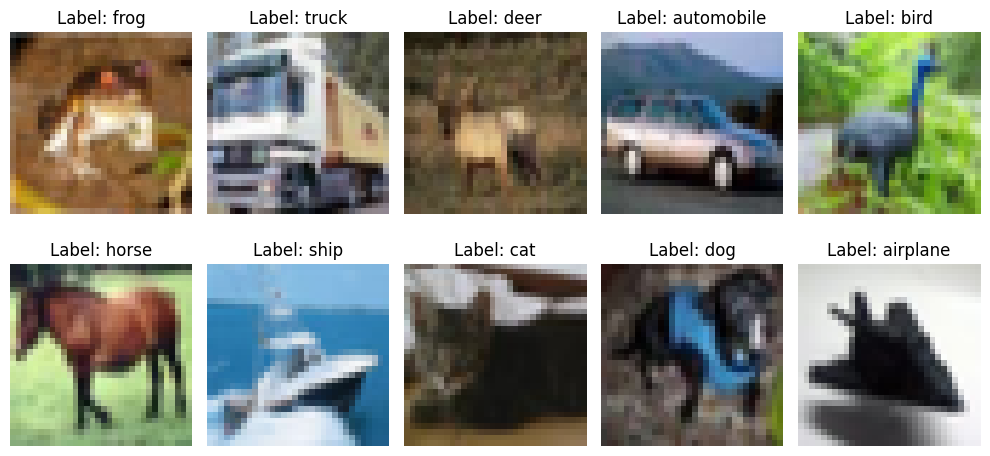
\includegraphics[width=0.75\textwidth]{imgplot.png}
        \caption{Plot showing one image for class of CIFAR10 dataset}
        \label{fig:imgplot}
    \end{figure}

    \newline The function \texttt{plot\_histogram} takes as arguments \texttt{classes}, the string label of each class, the trainset and the testset. In the \texttt{plot\_histogram} function I first initialize two dictionaries, one called \texttt{train\_counts=\{\}} which will contain the occurences of each class label in the trainset and \texttt{test\_counts=\{\}} which will contain the occurences of each class label in the testset. Then iterating on the labels of the trainset and on the label of the testset, i fill these dictionary having as key \texttt{classes[label]}, so the string label of the class, and as value the occurence, i.e. how many times an image of a certain class is encountered. To clarify, in the end we will have a dictionary structured as (e.g.) \texttt{\{'cat': 10, 'deer': 30,...\}} (this is an example, it doesn't reflect the real dataset values). Then I plot two different histograms having on x axis \texttt{dictionary.keys()}, the 10 classes labels, and on the y axis \texttt{dictionary.values()} so the number of images for each class. As we can see in Figure \ref{fig:trainHG}, in the trainingset - which, as I recall, is an istance of CIFAR10 dataset with \texttt{train=True} - we have $50.000$ images, $5000$ for each class. As we can see in Figure \ref{fig:testHG} in the testset we have $10.000$ images, $1000$ for each class.

    \begin{figure}[h]
        \centering
        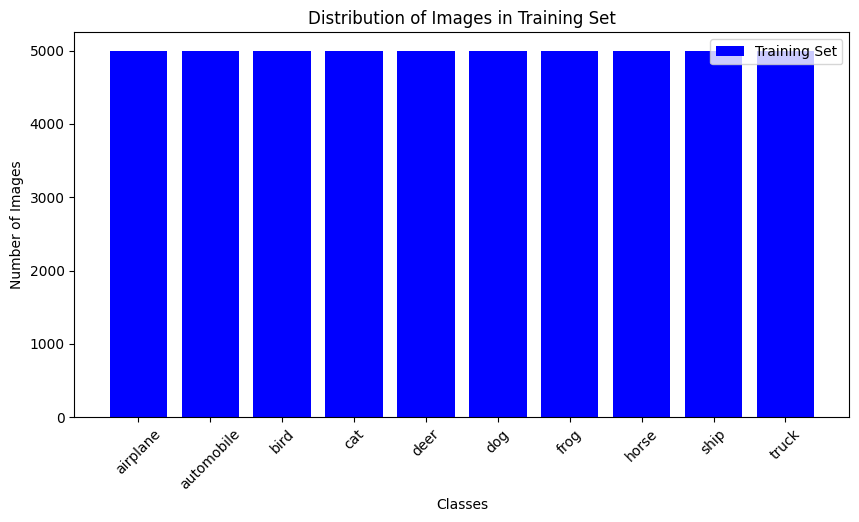
\includegraphics[width=0.75\textwidth]{trainingHG.png}
        \caption{Histogram of the distribution of images into classes of the training dataset}
        \label{fig:trainHG}
    \end{figure}

    \begin{figure}[h]
        \centering
        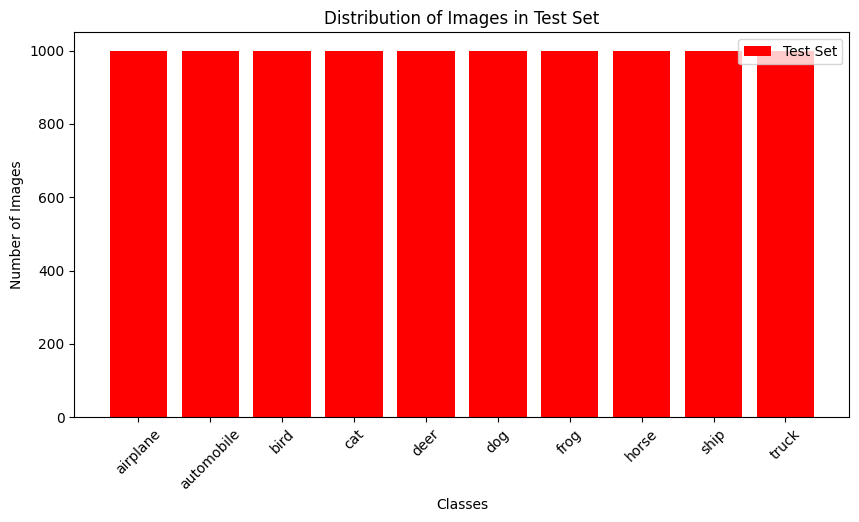
\includegraphics[width=0.75\textwidth]{testHG.png}
        \caption{Histogram of the distribution of images into classes of the test dataset}
        \label{fig:testHG}
    \end{figure}

	\item To arrive to a suitable format for a Deep Learning task, I need to transform each element of the dataset into a tensor. 
    \begin{itemize}
	    \item Please note that an element \texttt{data[i]} of the dataset is a tuple containing an \texttt{int} (the label) and a \texttt{PIL.image.Image}, which is an istance of the class Image representing a 32x32 RGB image.
        \item To convert this tuple into a suitable element, when istantiating the object of the \texttt{torchvision.datasets.CIFAR10} class, we can directly specify in the argument \texttt{transform=} what kind of transformation to perform onto the data. If I istanciate the new trainset object as \newline \texttt{trainset = torchvision.datasets.CIFAR10(root='./content/CIFAR-10', train=True,download=False, transform=transforms.ToTensor())}, I can obtain an istance of the class where each element is a tuple composed by a tensor (which is the image) and an integer label.
        \item  the size of the image as a tensor is a 32x32 input size with number of channels=3.
        \item This means that each image tensor contains 3 images of 32x32, one for each color channel. 
	\end{itemize}
	% Normalization
	\item In this step I increase the transformation operated onto the original dataset. To concatenate different transformation onto a data, I can use the function \texttt{transforms.Compose()}. This function allows me to perform different transformation onto the image and will come handful during the Data Augmentation procedure. The initial transformations that I apply on the CIFAR10 data are therefore:
    \begin{enumerate}
        \item \texttt{transforms.ToTensor()}: transforming the image into a \texttt{torch.Tensor} object
        \item \texttt{transforms.Normalize((0,0,0), (1,1,1))])} which basically applies normalization to the data with mean 0 and standard deviation 1 for each channel. Normalization basically rescales the features of the data to have a mean of 0 and a standard deviation of 1, which helps the model to better generalize.
    \end{enumerate}
	
	\item In this part of code I create a training set containing 80\% of the data and an evaluation set containing 20\% of the data. To do so I define a variable \texttt{train\_size=int(0.8 * len(trainset))}, which calculates how many samples correspond to 80\% of the totality of train data, and a \texttt{eval\_size=len(trainset) - train\_size} which basically measures to how many samples $1-80\%$ of the training data corresponds. Then I call the function \texttt{torch.random\_split} which given some inputs returns a tuple where the first element is the re-sized trainset and the second element is the evaluation set with the remaining samples. This function takes as arguments the trainset, the number of samples to assign to test and eval sets, and a \texttt{generator}. This generator is an istance of the \texttt{torch.Generator} class that basically generates random numbers in a reproducible way by specifying a seed ($42$ in this case). In this context it defines the randomical behaviour on which the sample will be assigned to trainset or evalset. In this section I also create 3 iterable istances, i.e. 3 batch loaders, one for the training set, one for the evaluation set, one for the test set. This will come handful for the training and testing pipeline. Batching onto the original dataset means to create batches or "subsets" of the original dataset on which the training pipeline can iterate. In easier words, with batching, the training loop, instead of iterating directly on each element of the dataset, it iterates on subsets of this datasets. Both for \texttt{trainloader}, \texttt{evalloader} and \texttt{testloader}  I set \texttt{batch\_size = 10}, the dataset is divided in batches of 10 samples. This means that, if for the training set we have $40.000$ samples, istead of directly iterating over the training set $40.000$ times, we iterate $4000$ times. I choose $10$ because it speeds up the convergence of the model to a suitable accuracy. For \texttt{trainloader} I set \texttt{shuffle=True}. Enable shuffling ensures that each batch is a random subset of the dataset. Without shuffling, consecutive batches would be contiguous subsets of the data, potentially leading to suboptimal training. Also, for each batch loader I defined \texttt{num\_workers=2}. Setting \texttt{num\_workers} to a value greater than 0 will create multiple worker processes to parallelize data loading
	
\end{enumerate}

\subsection{Model}
My model is defined as follows:
\begin{itemize}
    \item \textbf{Convolutional Layers:} I created 4 convolutional layers:
    \begin{enumerate}
        \item The first one takes an input with three channels (since we are working with RGB images), and applies $32$ filters with a kernel size of $3x3$ to each channel. The results from each channel are then summed to produce a single output value for a specific filter.Therefore applying $32$ filters will lead to an output channel of $32$.
        \item The second layer takes as input the output of the previous layer, so it has $32$ input channels and applies $64$ filters of kernel size $3x3$.
        \item The third layer takes $64$ input channels, applies $128$ filters of kernel size $3x3$
        \item The last convolutional layer takes $128$ input channels and applies $256$ filters of kernel size $3x3$.
    \end{enumerate}
    \item In all convolutional layers I choose \texttt{padding=1} and a $3x3$ kernel size. These are pretty standard choiches. Setting \texttt{padding=1} helps preventing information loss at the borders of the input. Padding creates an "external" row and column filled with $0$s. The main reasoning behind my choiches for the Convolutional setup of this Neural Network, lays in this note shared by the professor of Machine Learning, which basically said that " [...] in CNN we have learnable features, where convolutional layers play the role of \textbf{feature detectors} and pooling layers the role of \textbf{feature selectors}" My choiche of applying a high number of filters ($256$) was intended to allow my network to detect complex shared features between images. On the other hand, using a small (and pretty standard) kernel size ($3x3$) allows to reduce the number of learnable parameters (in comparison with higher kernel sizes) and therefore to obtain few highly complex shared feature. 
    \item \textbf{Pooling Layers:} I created one Max Pooling layer with $2x2$ kernel. As I will show in the forward step, this MaxPooling layer is applied to the input feature map after each two convolutional layers. MaxPooling divides the input into non-overlapping 2x2 regions and outputs the maximum value from each region. Thus, it reduces spatial dimensions, providing a downsized representation of the input. I choose MaxPooling instead of Average Pooling because I wanted to pick the most relevant shared features (also, AveragePooling performed worse than MaxPooling).
    \item \textbf{Fully Connceted Layers:} I use 3 fully connected layers:
    \begin{enumerate}
        \item The first one takes as input a flattened feature map (i.e. $256$x$1$) and transform it into a  $256 x 4$ tensor. Then returns a fully connected layer of output size $512$.
        \item The second fc layer takes as input size the ouput size of the previous layer and returns a fully connected layer of output size $256$.
        \item In the last fully connected layer the input size $256$ is shrunken to an output size $10$, which are the element we want to make predictions on (i.e. the 10 classes).
        These final feed forward layers take as input a shrunken feature map and parse it to make it suitable for predictions.
    \end{enumerate}
    \item \textbf{Forward Step: } in the forward step I apply the Relu activation function and a pooling of $2x2$ to the output of each convolutional layer. The Relu activation function is a non-linear function composed by two linear-parts. Is used to introduce non-linearity in the model, i.e. to allow the model to encode non-linear relationships between data, and thus to describe complex non-linear boundaries of decision. Important feature of this activation function are the sparsity property and the fact that it has no saturation effect (i.e. it mitigates the vanishing gradient effect). I use it beacuse it is one of the most common choiches in Convolutional Neural Networks and mainly because of the sparsity property: since Relu returns 0 for values $<=0$, it basically activates only neurons that describes relevant relationship between data, thus it focuses on relevant features and discard the less informative ones (at least this is what I initially thought, as I will show later). I applied pooling after each convolutional layer in order to create, at each step, feature maps that are as meaningful as possible and easy to manage due to their reduced size. I apply relu also on each fully connected layer (except the last one), where having non-linearity is recommended in order to have more manageable values. The \texttt{torch.flatten(x,1)} shrinks the output of the last pooling layer preserving the channel dimension. Basically it allows to describe the pooled feature map in a tensor  where each value corresponds to a specific channel in a specific spatial location. This makes it suitable for fully connected layers.  
\end{itemize}


\subsection{Training}
\begin{enumerate}
  	\item \textbf{Training Pipeline [lines 236-317]:} the training pipeline is similar to the one i described in the previous homework (where I perfomed training iterating on batches). I describe it in different steps to make the explanation more clear:
 \begin{itemize}
     \item I define the DEVICE (since I used only colab, I didn't inculde the code for checking Apple GPU). 
     \item I create an istance of the model and save it to the device.
     \item I define the loss function used. I choose \texttt{nn.CrossEntropyLoss()}. I choose this loss function because this model aims to perform a prediction task, so it is important to parse our results making them probabilistic. This criterion computes the cross entropy loss between input logits and target. 
     \item I set learning rate to $0.001$. This is a small step size for the optimizer, but it was the best performing of the ones I tried. I noticed that with small batch sizes ( I am using \texttt{batch\_size=10}), which may be linked to more noisy subsets of data, a small learning rate is preferable, as it tends to avoid getting stuck in sharp local minima and facilitates exploration of the parameter space.
     \item As optimizer I choose SGD, with m\texttt{momentum=0.9} and \texttt{weight\_decay=0}, which is the default. I choose SGD beacuse, in this model, it outperformed other optimizers such as \texttt{optim.Adam} (that was one of the most suggested for this kind of tasks). Momentum defines what proportion of past gradients to take into account to the current update in backpropagation. $0.9$ is a high momentum, as it takes into account almost 90\% of the past gradients.
     \item I declare two variables for storing evaluation and training loss at each epoch. I initialize loss with a really high value.
     \item I use $30$ epochs. With a small batchsize, the convergence is fast, so I don't need a lot of epochs. 
     \item \textbf{Training loop on batches.} I initialize \texttt{running\_loss = 0.0} and define the for loop onto the trainloader iterable. I perform a \texttt{enumerate} for loop so I can save in the variable \texttt{i} the step (or sub-batches) that have been considered. For each batch I save the inputs (images) and the labels it contains in two different variables, which are then saved in  the DEVICE. I set the parameters gradients to 0 with \texttt{optimizer.zero\_grad()}. I call the model on my inputs (in this case $10$ images) and save the outputs to the device. Outputs thus contains (in this case) $10$ estimated labels for $10$ input images. I compute the loss, i.e. Cross Entropy on estimated labels and real labels and then proceed to the backpropagation step. At each iteration I update the running loss, i.e. for each batch I compute the loss and add its value to the running loss variable. Each $2000$ batches considered, I print some statistics. More specifically, \texttt{\_, predicted = torch.max(outputs, 1)} returns the predicted class for each input in the batch, by looking at the maximum value of all elements in the input tensor. \texttt{correct = (predicted == labels).sum().item()} returns how much correct predictions were made, then \texttt{accuracy\_train = correct / batch\_size} basically returns the number of correct predictions divided by the total number of element of the batch. In short, if I have a \texttt{batch\_size=10}, for each batch I have $10$ images. \texttt{accurancy\_train} stores how much images were correctly labeled among all the $10$ images contained in the batch. Lastly, I print the epoch we are in, the number of batches considered, the loss and the accurancy.
     \item After each epoch I append the training loss to the \texttt{loss\_training} array.
     \item \textbf{Evaluation loop on batches.} After setting the model to \texttt{eval()} phase, I initialize the running loss and perform exactly the sam steps as for the training batch loop. The only noticeable difference is that in the evaluation phase we don't need to backpropagate, so we just compare the estimated labels with the real ones, compute loss and plot statistics. Monitoring the evaluation loss and accurancy is crucial for tuning your model. By looking at how it evolves you can make assumption on the choosen settings and how to change them to improve the model performance. 
 \end{itemize}
 
	\item \textbf{Compute Accurancy on the test set [lines 321-349]}: After the training and evaluation phase is concluded, I can run my model on a test set and compute its accuracy. The procedure is the same as for evaluation batch loop, but we do not need to compute loss. The final accuracy I get on $10.000$ unseen samples is: $72\%$. This means that this model, in 30 epochs returns an accuracy above $70\%$. 
	\item I save the model parameters in a ph file every $2000$ batches. The code is the following:
    \begin{lstlisting}
        PATH = '/content/MIOTTO_PIETRO_1.ph'
        torch.save(model.state_dict(), PATH)
    \end{lstlisting}
    \item As we can see in Figure \ref{fig:lossplot} the model is overfitting, because the training loss decreases while the evaluation loss increases. This means that my model is learning noise and is not generalizing enough to describe the relationship between samples and targets as a valid underlying structure. It may be worrying, but, in reality, I didn't take any explicit measure to reduce overfitting. 

    \begin{figure}[h]
        \centering
        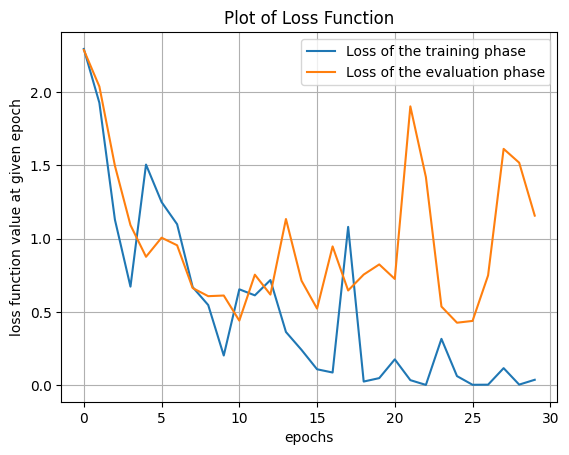
\includegraphics[width=0.75\textwidth]{Unknown-4.png}
        \caption{Plot showing the loss evolution between training set and evauation set}
        \label{fig:lossplot}
    \end{figure}

       	\item  I improve my model with the following:
 \begin{description}
     \item[Modification of the Model] I modified my model taking inspiration from \href{https://machinelearningmastery.com/how-to-develop-a-cnn-from-scratch-for-cifar-10-photo-classification/}{this article}. The main difference with the old model was that I stopped increasing the number of filters to $128$. Also, the model is deeper, since it uses $6$ Convolutional Layer instead of $4$. This model is a so called \textit{VGG Architecture}. VGG stands for Visual Geometry Group; it is a standard deep Convolutional Neural Network architecture with multiple layers. The “deep” refers to the number of layers, the most common implementations are  VGG-16 and VGG-19, consisting of 16 and 19 convolutional layers. The VGG architecture is the basis of ground-breaking object recognition models. The VGGNet it is one of the most popular image recognition architectures. In this simple classification task the article suggested to implement a \textit{VGG3}. The core of this architecture is to have two contiguous convolutional layers with the same output size. To clarify, the convolutional layers for VGG1 are defined as follows:
     \begin{lstlisting}
self.conv1 = nn.Conv2d(3, 32, 3, stride=1, padding=1)
self.conv2 = nn.Conv2d(32, 32, 3, stride=1, padding=1)
     \end{lstlisting}. 
     Thus with a VGG3 we get:
      \begin{lstlisting}
self.conv1 = nn.Conv2d(3, 32, 3, stride=1, padding=1)
self.conv2 = nn.Conv2d(32, 32, 3, stride=1, padding=1)
self.conv3 = nn.Conv2d(32, 64, 3, stride=1, padding=1)
self.conv4 = nn.Conv2d(64, 64, 3, stride=1, padding=1)
self.conv5 = nn.Conv2d(64, 128, 3, stride=1, padding=1)
self.conv6 = nn.Conv2d(128, 128, 3, stride=1, padding=1)
     \end{lstlisting}
Another difference with the old model is that \texttt{stride=1}, where the stride is the "step size" of the filter, i.e. "shift amount" between each step of the filter when it slides trough the image. In other words, the "stride" is the number of pixels the filter moves at each step. A larger stride value means that the filter skips more pixels when moving, resulting in a smaller output size and, since VGG is a deep convolutional network, potentially less computational cost. Consequently, the fully connected layers are reduced: VGG3 uses only two fully connected layers, the first takes as input a $128x4x4$ tensor and returns an output of $128$. The second reduces the input to $10$ predictions.
\item[Increase Batch Size [line 358]]: I increased the number of batches since with $10$ batches, on one side the model converges faster, but on the other its converges to a level of accuracy which lays around $75\%$, and doesn't actually get better. So I choose $32$ epochs, which slowed the convergence, but led to optimal results. 
\item[Data Augmentation [lines 351-357]] I also performed data augmentation on the training set (not on the test set of course). Data Augmentation is performed by appending to \texttt{transforms.Compose()} some image transformations that increase the variety (and variance) of data. With more noisy and variegated data the model should generalize better. I chained together the following transformations (please look at Figure \ref{fig:transf} for a better understanding):

        \begin{figure}[h]
            \centering
            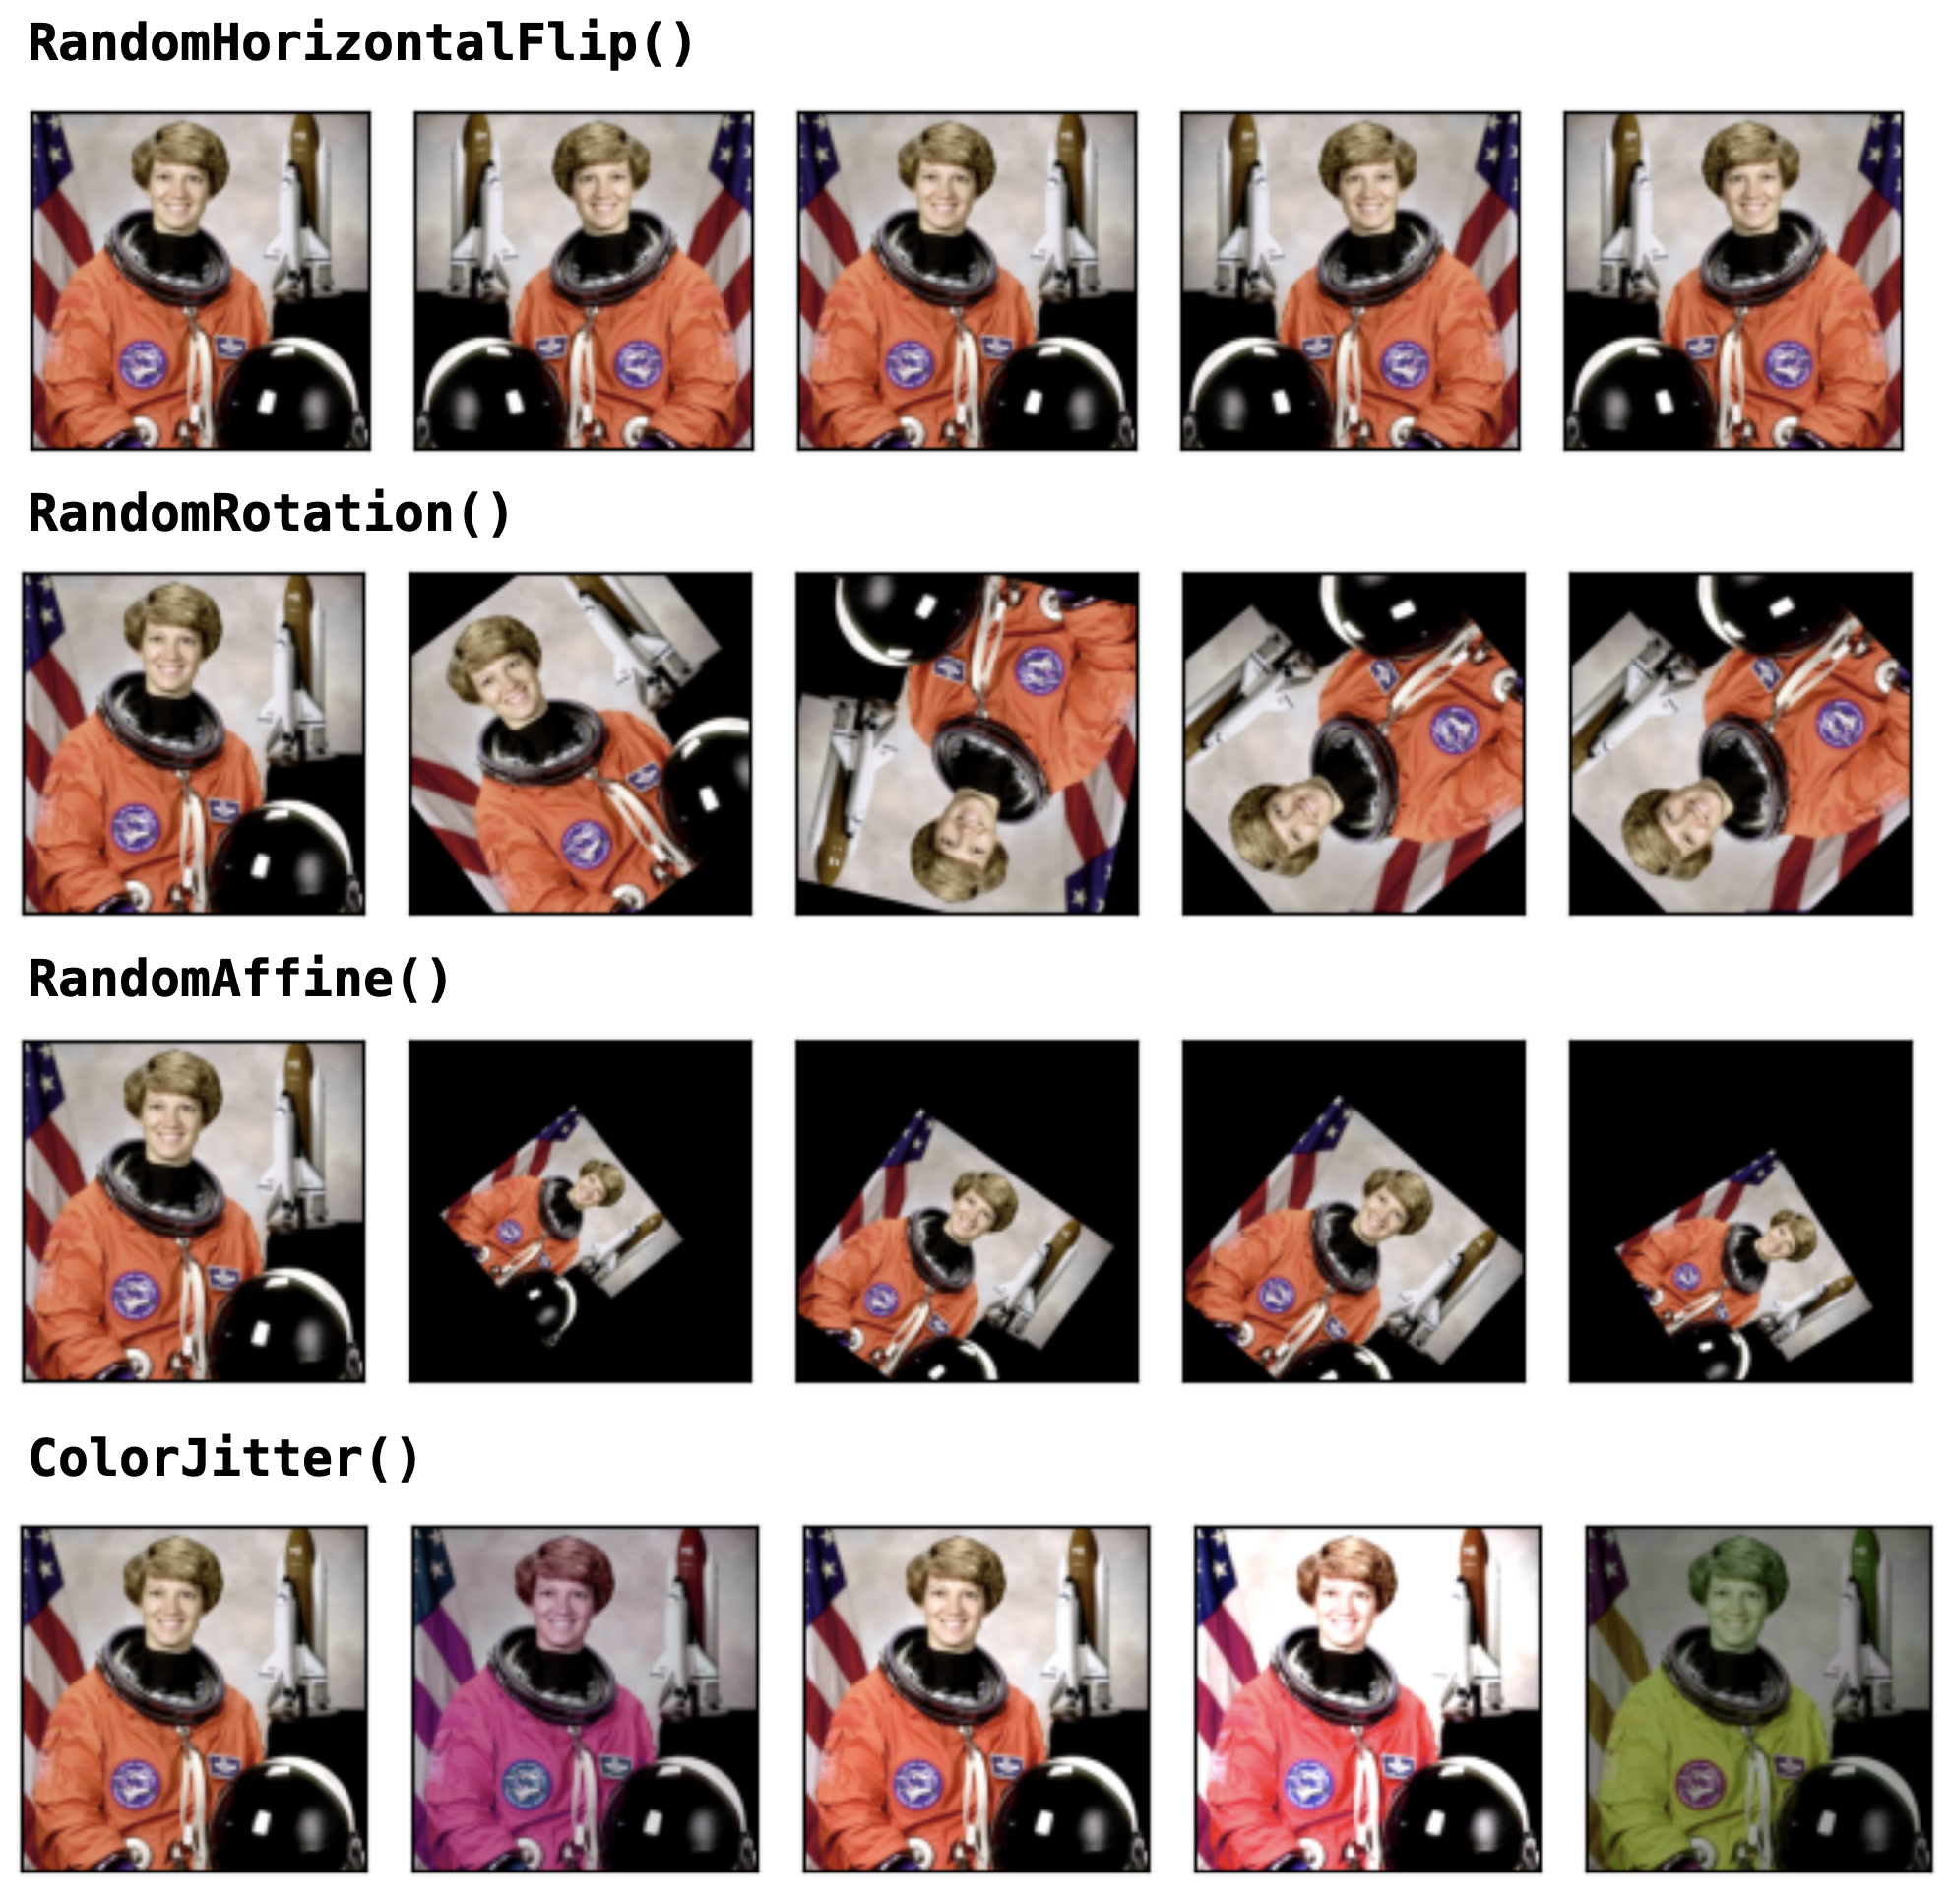
\includegraphics[width=0.75\textwidth]{transformations.png}
            \caption{Different transformation applied to perform data augmentation. Examples taken from \href{https://pytorch.org/vision/main/auto_examples/transforms/plot_transforms_illustrations.html#sphx-glr-auto-examples-transforms-plot-transforms-illustrations-py}{pytorch documentation}}
            \label{fig:transf}
        \end{figure}

       \begin{itemize}
    \item \texttt{RandomHorizontalFlip()}: This transformation randomly flips the input image horizontally with a 50\% probability. Suppose most of the cat images show the animale facing left. By applying this transformation, the dataset would consist of more images of cat facing right.
    \item \texttt{RandomRotation(10)}: This transformation randomly rotates the input image using a degree in the range $[-10; 10]$.
    \item \texttt{RandomAffine(0, shear=10, scale=(0.1, 1.2))}: to understand this transformation I suggest you to look at \ref{fig:transf}. It is pretty complicated to explain.
    \item \texttt{ColorJitter(brightness=0.2,contrast=0.2, saturation=0.2)} This transformation randomically increases/decreases brightness, contrast and saturation of the images. 
\end{itemize}
\item[LeakyRelu]: I used \texttt{nn.LeakyReLU(negative\_slope=0.1)} which is basically a RELU activation function but with a negative slope, i.e. the negative inputs are not directly set to $0$, but they follow a sligthly negative slope. Basically, Leaky ReLU allows a small, non-zero gradient for negative inputs. I decided to use this activation function because, since even neurons with negative inputs contribute to the learning process, I wanted to not arbitrarily deactivate all neuron that returns values $<= 0$.
\item[Adding Dropout] I added dropout after each pooling layer (which in VGG is performed every two convolutional layers). Dropout basically deactivate neurons randomically, drastically reducing overfitting. I set \texttt{Dropout=0.5}, which means that half of the neurons are deactivated at each step. Deactivating neurons prevents the network from relying too much on specific neurons and forces it to learn more robust and generalized features. This, with data augmentation, was sufficient to reduce overfitting of the model (I didn't need to use weight decay).
\item[Adding BatchNormalization]: I added Batch Normalization to each Convolutional Layer.Batch Normalization basically normalizes the inputs of each layer, speeding up the convergence. Since I increased the batch size (and so the time the model takes to converge), introducing batch normalization astonishingly sped up the process: firstly it took me more than $100$ epochs to reach $81\%$ accuracy, with batch normalization it took only $50$ 

        \item[Increase Epochs [line 380]:] I tried different batch sizes with different epochs. With this learning rate I noticed that the higher the batch size, the slower the convergence and, up to some point, the optimal the results. I tried a wide variety of epochs, in increasing order. In Figure \ref{fig:epoch} is it possible to see how a certain number of epochs led to a certain amount of accuracy (in this case the image refers to using \texttt{batch\_size=32}).

        \begin{figure}[h]
            \centering
            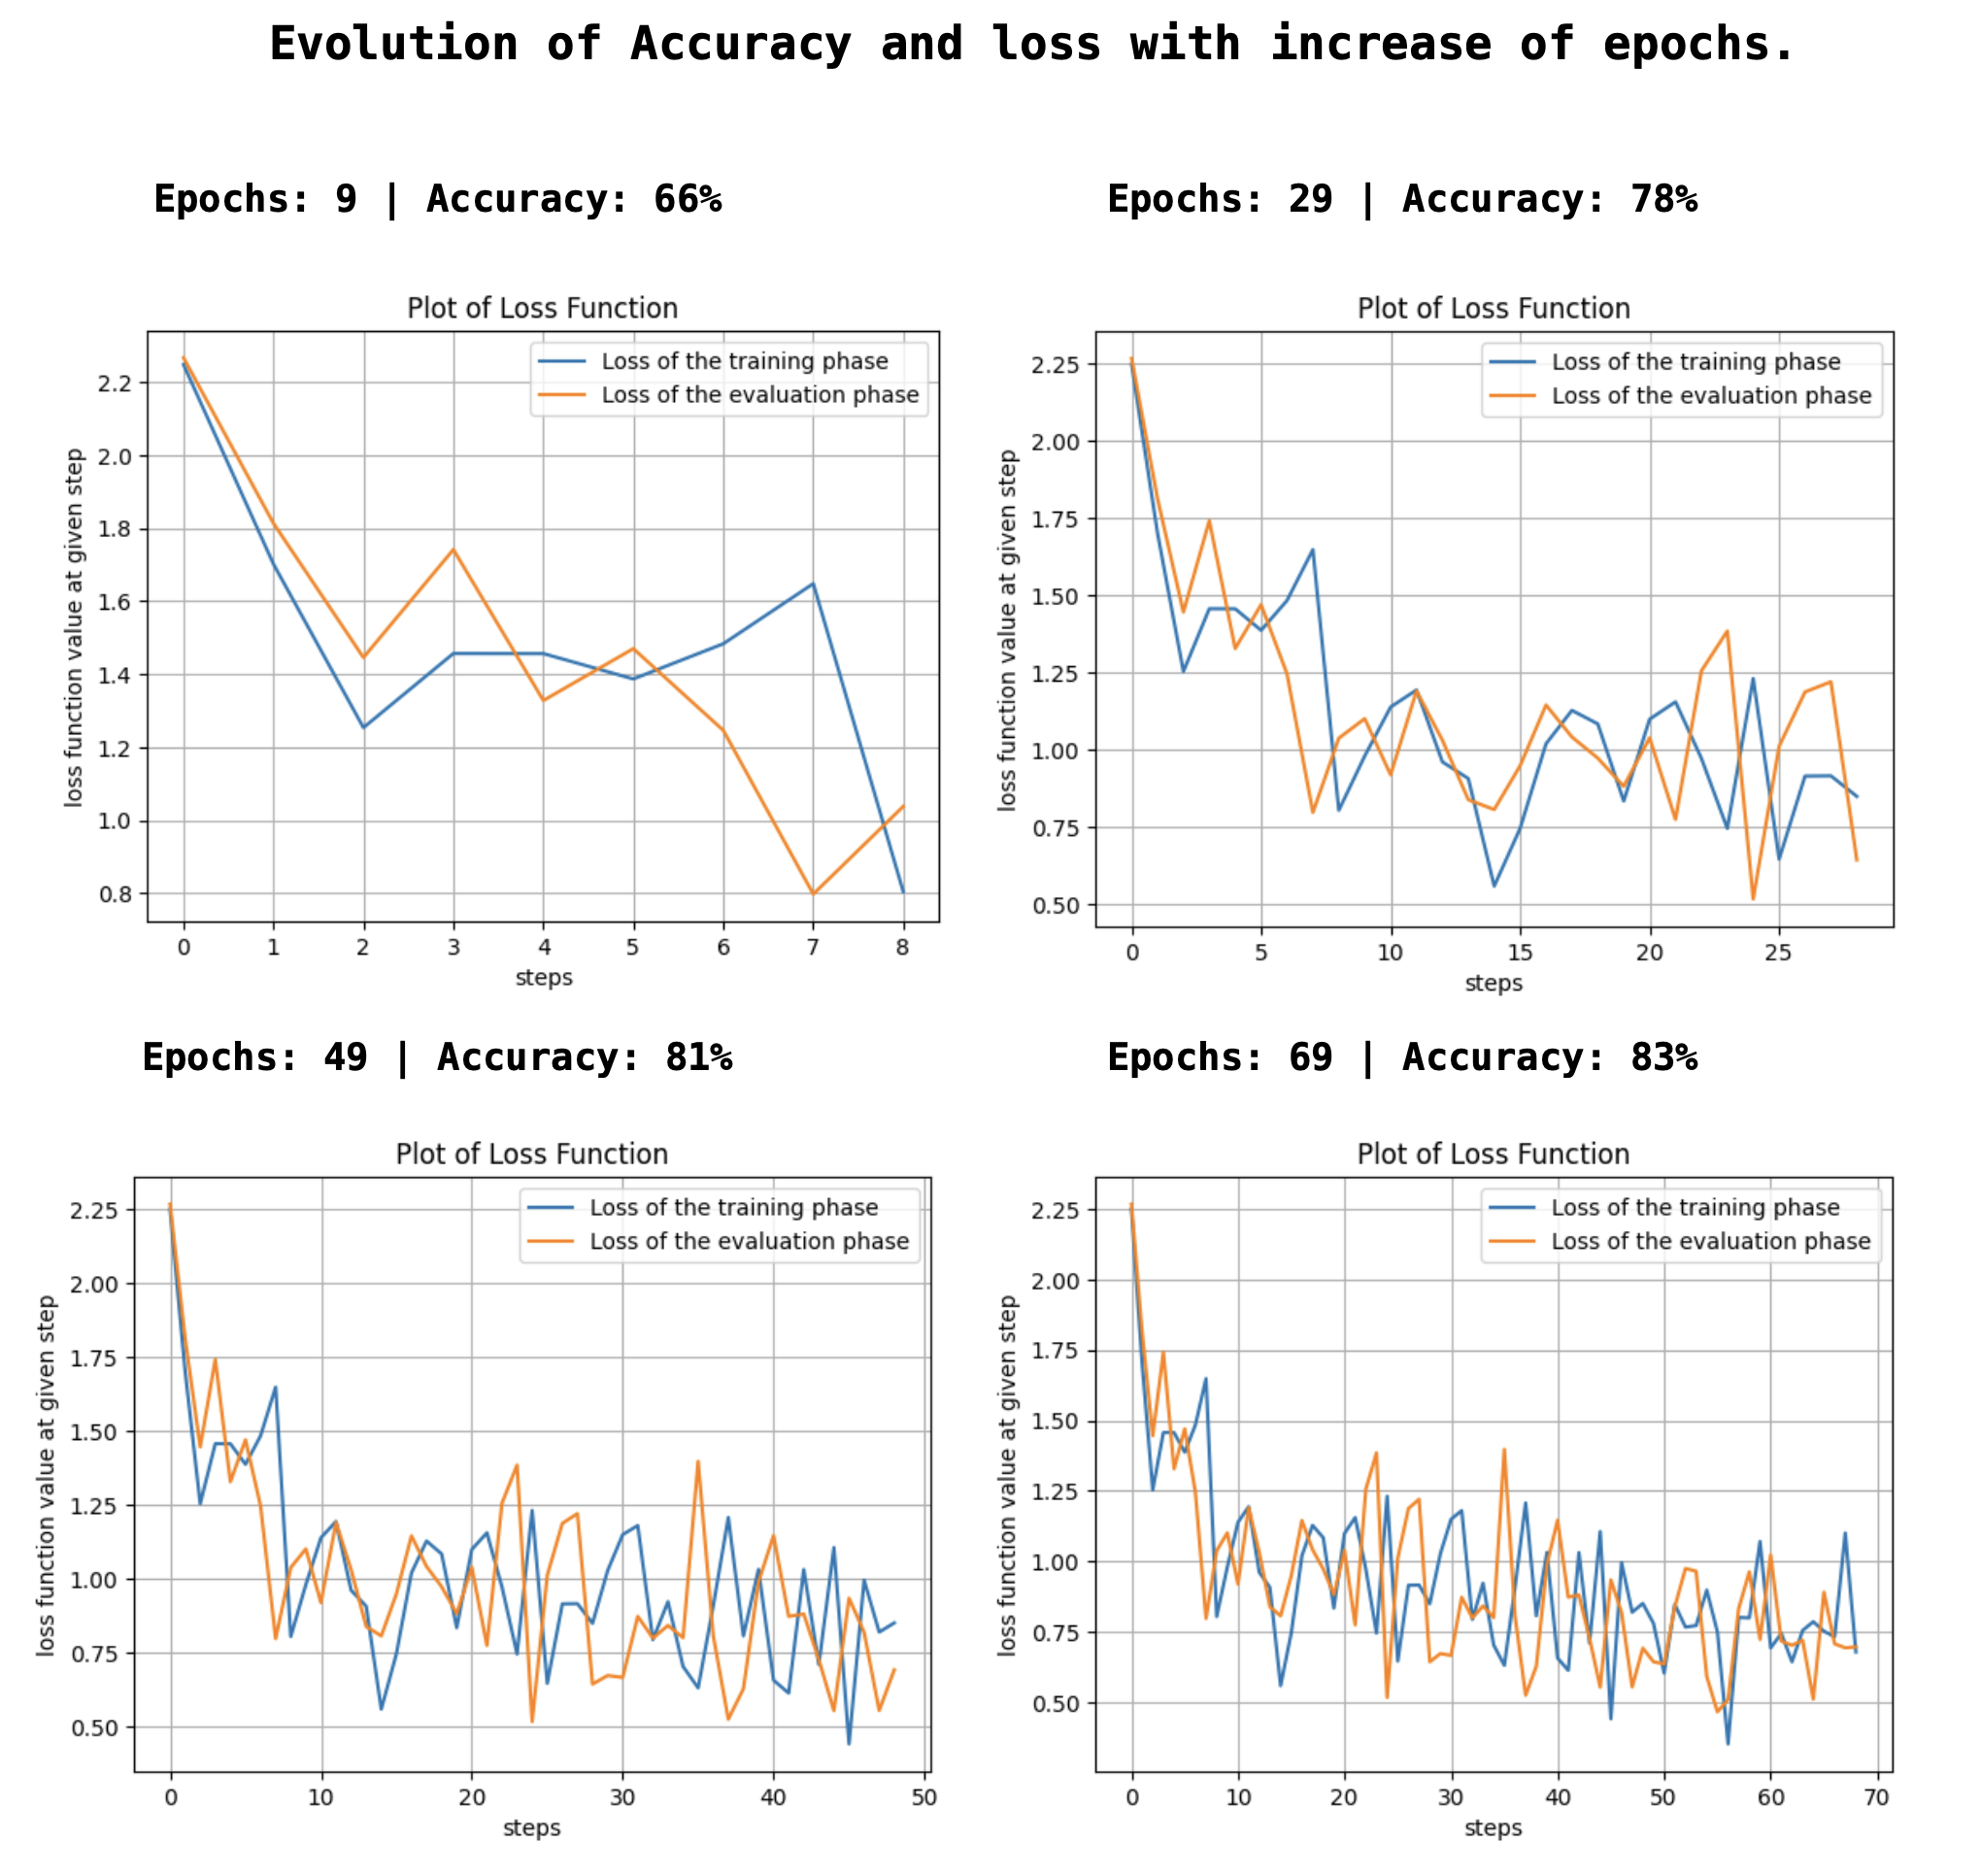
\includegraphics[width=0.75\textwidth]{epoch.png}
            \caption{Evolution of evaluation and trainig loss, as well as evolution of accuracy related to increase of epochs with batch size 32. \textit{Please note that the label "step" here refers to epochs. }}
            \label{fig:epoch}
        \end{figure}
    \end{description}

\item The Model parameters are saved in this line of code [lines 440-441]:
 \begin{lstlisting}
PATH = '/content/MIOTTO_PIETRO_2.ph'
torch.save(model2.state_dict(), PATH)
 \end{lstlisting}
\end{enumerate}

\end{document}